\documentclass[11pt,twoside]{uhthesis}
\usepackage{subfigure}


\title{Automatizar la creación de Generadores Multilenguajes}
\author{Yasmany Arcia Corcho}
\advisor{MSc. Fernando Rodríguez Flores}
\degree{Licenciado en Ciencia de la Computación}
\faculty{Facultad de Matemática y Computación}
\date{Mayo 2017}
\logo{Graphics/uhlogo}
\makenomenclature

%%%{{{ Comments and the like
\usepackage[textwidth=4cm]{todonotes}
\usepackage{soul}
\newcounter{todocounter}
\newcommand{\comment}[2]{\stepcounter{todocounter}
  {\color{green!50!blue}{(#1$^{{\color{black}\textbf{\thetodocounter}}}$)}}
  \todo[color=green,noline,size=\tiny]{\textbf{\thetodocounter:} #2

  }}
\newcommand{\quitaesto}[1]{{\color{red}(\st{#1})}}

\newcommand{\cambio}[2]{{\color{cyan}{{#2}}}{\color{red}{(\st{#1})}}}

\newcommand{\agregaesto}[1]{{\color{cyan}{{#1}}}}

\newcommand{\errorortografico}[1]{{\fcolorbox{gray}{magenta}{\textcolor{yellow}{\bf #1}}}}

\newcommand{\primerapersona}[1]{{\fcolorbox{gray}{green}{\textcolor{yellow}{\bf #1}}}}

\newcommand{\vozpasiva}[1]{{\fcolorbox{gray}{blue}{\textcolor{yellow}{\bf #1}}}}
    
%%%}}}

\newcommand{\gagm}{MGA}

\begin{document}
\frontmatter
\maketitle
\parskip = 5pt

\begin{dedication}
\emph{A mi mamá por su confianza, \\su infinita dedicación y su \\amor
incondicional.} 
\end{dedication}
\begin{acknowledgements}
Agradezco especialmente a mi Mamá y a mi familia. 
A mi tutor Fernando y a su mamá por su dedicación y apoyo.
A todas las personas que forman parte importante de mi vida.         
\end{acknowledgements}
\begin{opinion}
En los últimos años he sido testigo del desarrollo de varios ``Generadores
Multilenguajes'' (como son llamados en este documento) y yo mismo he
desarrollado algunos.  A cada uno de ellos le tomó un par de meses llegar
a un estado medianamente funcional, y un poco más de un semestre para ser
realmente útil.  Con el trabajo que se defiende en este documento de
tesis, esos tiempos se pueden reducir a un par de días y un par de
semanas, respectivamente.  Eso es posible gracias al trabajo de Yasmany.

Durante la realización de este trabajo Yasmany mostró una excelente
capacidad de abstracción, habilidades en la detección y solución de
problemas, y capacidad para asimilar nuevos lenguajes de programación y
nuevas formas de pensar, completamente diferentes a las adquiridas durante
las asignaturas de la carrera.

Creo que estamos en presencia de un excelente trabajo que evidencia que
Yasmany Arcia Corcho reúne todos los requisitos para desempeñarse como un
excelente graduado de Ciencia de la Computación.
\end{opinion}
\begin{abstract}
La implementación de un Lenguaje de Dominio Especifico (DSL) requiere diseñar un programa capaz de leer líneas de texto escritas en dicho DSL, analizarlas, procesarlas y hacer posible su generación de código o implementación hacia otros lenguajes. En dependencia de su propósito, desarrollar un DSL puede necesitar varias etapas, pero la mayoría de estas fases son comunes en todas las implementaciones. En este trabajo se presenta una herramienta para automatizar la creación de DSLs que generen códigos hacia múltiples lenguajes. Dicha herramienta permite a los desarrolladores abstraerse de la implementación de analizadores lexicográficos y semánticos, automatizar la construcción de los nodos del Árbol de Sintaxis Abstracta del lenguaje a diseñar y simplificar la generación de código a los lenguajes que se desee exportar.
\end{abstract}


\begin{englishabstract}
The implementation of a Specific Domain Language (DSL) requires designing a program capable to read lines
of text written in that DSL, analyze and process them and make possible its code generation or implementation
into other languages. Depending on the purpose of the DSL, developing it may need several stages, but most of
these stages are common in all implementations. This paper presents a tool to automate the creation of DSLs
that generate codes into multiple languages. This tool allows developers to abstain from the implementation
of lexical and semantic analyzers, automate the construction of the Abstract Syntax Tree nodes of the
language to be designed and simplify the code generation of the languages to be exported.	
\end{englishabstract}
\tableofcontents
%\listoffigures
%\listoftables

\mainmatter
\begin{introduction}
  
Un lenguaje de dominio específico (DSL, por sus siglas en ingl\'es) es un conjunto de construcciones y operaciones que brindan una mayor expresividad para representar soluciones de un dominio en particular \cite{dslEngineering}. Los DSLs pueden ser internos en un lenguaje de programaci\'on o externos \cite{dsl1}. Algunos ejemplos de DSLs son: BNF (\textit{Backus Normal Form}) para describir la sintaxis de los lenguajes de programaci\'on \cite{BFN}; Matlab \cite{matlab}, utilizado para el trabajo con matrices, y el lenguaje de programaci\'on R, diseñado por estad\'isticos y para estad\'isticos \cite{R}. Por lo general, a partir de programas escritos en estos DSLs, se genera el código ejecutable de los mismos, o se transforman en código fuente de un lenguaje de programación específico y este último se compila \cite{dslEngineering} \cite{implementations_DSL} \cite{dsl1}. 

Para el diseño e implementaci\'on de DSLs, se pueden usar herramientas como {DSL Tools} para la plataforma .NET \cite{dsltools} y el framework XText de Java \cite{xtext}. 

Existen escenarios en los que se desea representar en distintos formatos (o lenguajes de programación) el código de programas escritos en un DSL específico. Por ejemplo, cuando se quiere representar el mismo documento en varios formatos como HTML \cite{HTML} y PDF \cite{pdf}, o cuando se desea obtener el código fuente en varios lenguajes de programación de bibliotecas de Diferenciación Automática implementadas en un DSL \cite{Da}. Para el primer escenario, existen aplicaciones como TexInfo \cite{texinfo}, {Markdown} \cite{markdown}, y el Modo Org de Emacs \cite{emacs}, que a partir de la representación de un documento en un lenguaje de marcado específico,  permiten obtenerlo en varios formatos; y para el segundo escenario, existen aplicaciones como ADOL* \cite{Adol*}. Este tipo de herramientas constituyen el objeto de estudio de este trabajo, y serán llamadas Generadores Multilenguajes.

Un Generador Multilenguaje es una aplicación que define un DSL, y permite representar en múltiples formatos los programas escritos en \'el. Dichos  formatos serán llamados lenguajes de salida. Para construir un Generador Multilenguaje, es necesario diseñar e implementar un DSL que represente su dominio y posteriormente especificar c\'omo se escribe cada componente del DSL en los lenguajes de salida.

En los \'ultimos años, en la Facultad de Matemática y Computaci\'on de la Universidad de La Habana (MATCOM) se han desarrollado Generadores Multilenguajes en varios dominios como \emph{ADOL*} para la creaci\'on de bibliotecas de Diferenciaci\'on Autom\'atica;  \emph{LAML} que permite expresar modelos de programación matemática \cite{hoyos}; y un lenguaje para la descripción de criterios de vecindad en problemas de enrutamiento de vehículos (IVNS) \cite{cami}. Todas estas aplicaciones se han implementado como DSLs internos en el lenguaje de programación Common Lisp, aprovechando la notación infija del mismo, y utilizando como palabras clave del DSL los constructores de las clases que representan los nodos de los posibles \'Arboles de Sintaxis Abstracta (ASTs).


%Actualmente, se est\'a desarrollando dos proyectos en esta misma l\'inea: un lenguaje de modelaci\'on algebraico para problemas de optimización [tesis de hoyos] y un lenguaje para describir criterios de vecindad en algoritmos de b\'usqueda local para problemas de enrutamiento de veh\'iculos [ref camila]. 



En la construcción de un Generador Multilenguaje se puede identificar un conjunto de pasos necesarios para el desarrollo del mismo:

\begin{enumerate}
	\item Determinar el dominio que se quiere representar en el DSL.
	\item Identificar los elementos que se desean representar en el DSL.
	\item \label{item:diseñar-dsl} Dise\~nar el lenguaje del DSL.
	\item \label{item:jerarquia-de-clases}Implementar una jerarqu\'ia de clases que permita representar cada uno de los elementos del DSL como nodos de un AST.
	\item \label{item:paso-parser-lexer} Construir el analizador lexicogr\'afico y el sint\'actico.
	\item 	\label{item:generacion-de-codigo}Implementar la generaci\'on de c\'odigo de cada uno de los nodos del AST, en cada uno de los lenguajes de salida.
  \end{enumerate}

  Cuando el DSL del Generador Multilenguaje es un lenguaje interno de Common Lisp, el paso \ref{item:diseñar-dsl} se convierte en una selección apropiada de nombres para los constructores de las clases del AST, y el paso \ref{item:paso-parser-lexer} no es necesario, pues este proceso lo realiza el intérprete de Lisp. Además, los pasos \ref{item:jerarquia-de-clases} y \ref{item:generacion-de-codigo} se pueden automatizar utilizando macros y el Sistema de Objetos de Common Lisp.

  La principal contribución de este trabajo es la propuesta de una nueva herramienta en Common Lisp, denominada Automatización de Generadores Multilenguajes (\gagm\footnote{Multi-languages Generators Automation}), para la automatización de los pasos \ref{item:jerarquia-de-clases} y \ref{item:generacion-de-codigo} en la creación de Generadores Multilenguajes en Common Lisp. Esto se traduce en automatizar el proceso de creación de las clases para representar los elementos del dominio como nodos de un AST y simplificar la generación de código de cada uno de estos nodos en los diferentes lenguajes de salida.

Para desarrollar este trabajo fue necesario estudiar el diseño e implementación de DSLs, elementos de compilación y el lenguaje de programación Common Lisp. Dichos elementos se presentan en el Capítulo \ref{chap:basis}. Independientemente del lenguaje de programación donde se desee implementar un Generador Multilenguaje, los pasos para construirlo son similares. En el Capítulo \ref{chap:implementacion de un generador } se ilustran sus pasos a través de la definición de BASAR, un Generador Multilenguaje orientado al trabajo con operaciones aritméticas. El Capítulo \ref{chap:GAGM} está dedicado a presentar como se pueden implementar estos programas en Common Lisp, a encontrar patrones de código que se repiten en este proceso; y se presentan los macros \texttt{defnode} y \texttt{gcode}, cuyo uso elimina el código que se repite. El código que generan los macros \texttt{defnode} y \texttt{gcode} es completamente modificable como se muestra en el Capítulo \ref{chap:GAGMA}. Finalmente se presentan las conclusiones, recomendaciones y la bibliografía consultada.


\end{introduction}
%%% Local Variables:
%%% mode: latex
%%% TeX-master: "../Thesis"
%%% End:

 \chapter{Preliminares}
\label{chap:basis}

En este capítulo se presentan los elementos fundamentales para el desarrollo de este trabajo. En la sección \ref{sec:definiciones-basicas} se presenta un conjunto de definiciones que serán utilizadas a lo largo del documento. Las otras secciones están dedicadas a las herramientas necesarias para automatizar la construcción de Generadores Multilenguajes en Common Lisp, que constituye el objetivo principal de este proyecto. Estas herramientas son: los Lenguajes de Dominio Específico (DSL), los Árboles de Sintaxis Abstracta (ASTs) y, por último, el lenguaje de programación Common Lisp, en el cual está implementada la herramienta propuesta en este trabajo.

\section{Definiciones básicas}
\label{sec:definiciones-basicas}

En la computación, existen diversos lenguajes para representar un problema de un área en particular. Esto obliga a los desarrolladores a escribir la misma solución en cada lenguaje donde desee emplearla. Un camino para simplificar el trabajo de los programadores en esta situación, sería implementar la solución en un Generador Multilenguaje.


\begin{definition}
  Un Generador Multilenguaje es una aplicación que define un DSL, y permite que los programas escritos en él puedan ser representados o exportados a varios lenguajes.
\end{definition}


Ejemplos de Generadores Multilenguajes son: Markdown \cite{markdown} y ORG-Mode \cite{emacs} que se especializan en exportar documentos a distintos formatos como HTML \cite{HTML}, LaTeX \cite{latex}, u ODT \cite{ODT}, a partir de un lenguaje de marcado que ellos definen; ADOL* es implementado en Common Lisp para representar Rutinas de Diferenciación Automática en varios lenguajes de programación \cite{Adol*}; Problemas de enrutamiento de vehículos (IVNS) \cite{cami}; Problemas de programación matemática (LAML) \cite{hoyos}.

\begin{definition}
  El dominio de un Generador Multilenguaje es el área de trabajo en que se especializa.
\end{definition}

El dominio de ADOL* es la Diferenciación Automática; el de Markdown, la edición de documentos; y el de LAML, los modelos de programación matemática \cite{hoyos}. 

\begin{definition}
	Un elemento del dominio representa una parte específica del área de trabajo.
\end{definition}

Algunos elementos en el dominio de Markdown son los textos, las listas de viñetas, y las referencias a documentos. En el dominio de (IVNS) se pueden encontrar los vehículos, los criterios de vecindad y las posibles rutas para los vehículos.

\begin{definition}
 Un lenguaje de salida es un lenguaje en el cual se desea representar los programas escritos en un Generador Multilenguaje.
\end{definition}

Entre los lenguajes de salida de Markdown se encuentran HTML, LaTeX, y ODT \cite{ODT}. En el caso de ADOL*, un lenguaje de salida, es cualquier lenguaje de programación que posea sobrecarga de operadores.   
 \begin{definition}
 Un Generador Multilenguaje es extensible si permite agregar nuevos lenguajes de salida.
 \end{definition}

 ADOL*, ORG-Mode y Markdown constituyen Generadores Multilenguajes extensibles. ADOL* permite agregar cualquier lenguaje de programación con sobrecarga en los operadores. ORG-Mode define una interfaz para implementar nuevos exportadores.


\section{Lenguajes de Dominio Específico}
Los ingenieros de software se encargan de encontrar herramientas para representar soluciones a problemas de las ciencias computacionales. Unas de las principales tendencias para la creación, modernización y mantenimiento de programas es el modelado de dominio especifico (\emph{DSM}) \cite{DSM}. Esta técnica propone crear abstracciones de los problemas para que los usuarios expresen fácilmente sus soluciones y ha sido utilizada en el desarrollo de lo que se conoce como Lenguajes de Dominio Específico (DSL). 

Un DSL es un lenguaje de programación destinado a aumentar la productividad de los usuarios al resolver un problema dentro de un contexto específico \cite{implementations_DSL}. Estos tienen la característica de ser típicamente más pequeños que los lenguajes de propósito general, pero al complementarse con otros ambientes de producción brindan un mejor nivel de abstracción sintáctico y semántico para la representación de un problema, permitiendo de esta forma ocultar las complejidades que aparecen en el proceso. Precisamente por ese motivo, y porque las herramientas actuales permiten crear nuevos lenguajes de programación con relativa facilidad, el uso de los DSLs es cada vez más frecuente \cite{dsl1}

En las siguientes secciones se presentan características de los DSLs relevantes para este trabajo: si son externos o internos y las etapas en su construcción.

\subsection{DSLs internos o externos}
Desde el punto de vista de la construcción del lenguaje, los DSLs se pueden clasificar en \textit{internos} o \textit{externos}. Los \textit{internos} forman parte de la sintaxis de un lenguaje de propósito general existente, usualmente en forma de librerías. Entre ellos se pueden mencionar Rails (construido en Ruby) \cite{ruby} y {ASP.NET Core} \cite{asp.netcore}, ambos orientados al desarrollo de aplicaciones web; el Sistema de Objetos de Common Lisp (CLOS) \cite{sonya} y Entity Framework \cite{entity}, un ORM (por sus siglas en inglés Object Relational Mapping) para .NET.
 
Los \textit{externos} se caracterizan por tener su propia sintaxis. Producto de que son construidos desde cero, estos tienen una sintaxis más especializada que los internos, pero requieren de la construcción de un compilador. Algunos ejemplos son {MATLAB}, para el trabajo con matrices y cálculos científicos \cite{matlab}; Graphviz, orientado al dibujo de grafos \cite{graph}, y R, cuyo propósito es brindar un lenguaje de programación orientado al trabajo estadístico \cite{R}.

\subsection{Construcción de un DSL}

En la literatura sobre Lenguajes de Dominio Específico se han identificado cinco etapas en la construcción de un DSL: \textit{Decisión}, \textit{Análisis}, \textit{Diseño}, \textit{Implementación} y \textit{Despliegue} \cite{dslEngineering} \cite{implementations_DSL} \cite{dsl1}.

En la etapa de \textit{Decisión} se investiga si es factible o no crear un DSL para el dominio seleccionado; posteriormente, en la etapa de \textit{Análisis} se investigan los elementos necesarios para modelar dicho dominio. Durante la etapa de \textit{Diseño}, se elige un lenguaje de programación en el cual implementar el DSL y se considera qué patrón de diseño utilizar \cite{dslEngineering}. Terminadas las etapas anteriores, corresponde la etapa de Implementación del DSL. Por último, se desarrolla la etapa de \textit{Despliegue}, que según Meyer \cite{meyer}, es la etapa más compleja durante la vida útil de un software.

En este trabajo, se implementó una herramienta para diseñar DSLs internos en Lisp, asumiendo que las etapas de \textit{Decisión}, \textit{Análisis} y \textit{Diseño} para la creación de un DSL están cumplidas correctamente. En la siguiente sección se presentan los {Árboles de Sintaxis Abstracta}, que resultan vitales para la etapa de Implementación de un DSL, y para la generación de código en los Generadores Multilenguajes.

\section{Árbol de Sintaxis Abstracta }
Un Árbol de Sintaxis Abstracta (AST, por sus siglas en inglés) es una estructura arbórea utilizada para representar segmentos de código escritos en programas computacionales.  Cada nodo del árbol contiene información recolectada durante el análisis lexicográfico y el sintáctico de un programa específico \cite{AST}. En la figura \ref{AST1} se muestra un AST correspondiente a la expresión $X= (Y+2) * (Z+3)$.  
Nótese que han sido eliminados los paréntesis y el punto y coma.

\begin{figure}
	\centering
	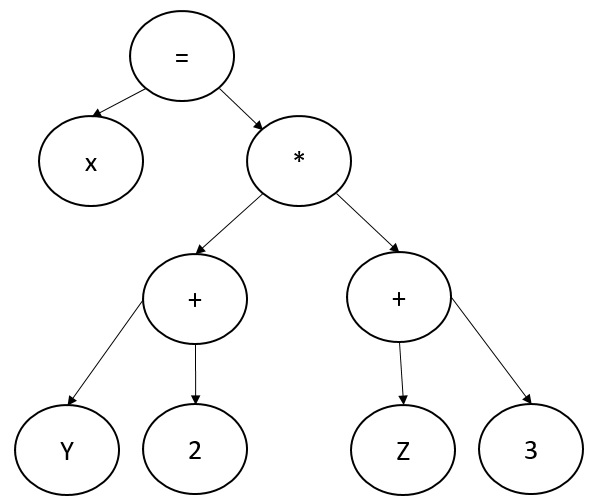
\includegraphics[width=0.6\textwidth]{AST1.png}
	\caption{AST correspondiente a la expresión: $X = (Y+2) * (Z+3);$}
	\label{AST1}
\end{figure}


Los nodos de un AST suelen ser instancias de clases diseñadas para representar cada operación del lenguaje, de forma que estos almacenen información necesaria de los elementos del dominio de un lenguaje de programación \cite{AST}. 

En {\gagm}, para generar el código fuente de un programa escrito en un DSL en cualquier lenguaje de programación, es necesario obtener el AST correspondiente. Para cumplir este objetivo, existen herramientas como ANTLR \cite{antlr} y YACC \cite{yacc}, aunque no siempre es necesario utilizarlas. Por ejemplo, en lenguajes como Ruby \cite{ruby} o Common Lisp \cite{clos-overview}, cuando el DSL que se está desarrollando es interno, no se requiere el uso de ninguna de las herramientas existentes para crear el AST de un programa, porque estos lenguajes brindan recursos propios, los cuales resultan más convenientes para la creación de este tipo de DSL. Además, como el objetivo de este trabajo es automatizar el proceso de Generadores Multilenguajes en Lisp, no es necesario realizar el análisis léxicográfico y sintáctico porque el intérprete de Lisp realiza esta tarea. La próxima sección está dedicada al lenguaje de programación Common Lisp.

\section{Common Lisp}

LISP es un lenguaje de propósito general creado en los años 50 por John McCarthy y fue desarrollado con el objetivo de crear un lenguaje que mostrara la información estructurada en listas, de ahí su nombre List-Processing \cite{ansi-common-lisp}.  Es el segundo lenguaje de alto nivel más antiguo que aún se utiliza en la actualidad, después de Fortran \cite{gentle-introduction-to-common-lisp}. La variedad de dialectos Lisp existentes en 1981 (Maclisp, Interlisp, zetalisp), provocó que en 1986 se creara el estándar llamado Common Lisp \cite{Land-of-Lisp}.

%Algunos de los escenarios en los cuales se emplea actualmente son La Inteligencia Artificial [paradig-lip] y el Procesamiento de Lenguaje Natural [natural proc lang in lisp].

Common Lisp es un lenguaje multiparadigma. En él, es posible crear programas orientados a objetos \cite{sonya}, completamente funcionales \cite{onlisp}, o cualquier combinación que se desee \cite{Land-of-Lisp}.  Posee un intérprete interactivo conocido por sus siglas REPL \cite{practical-common-lisp} y un Sistema de Objetos (CLOS) basado en herencia múltiple y funciones genéricas \cite{sonya}.

Las características que distinguen a Common Lisp del resto de los lenguajes de programación son su Sistema de Objetos y un Sistema de Macros que permite modificar el lenguaje para ajustarlo a las necesidades del usuario \cite{practical-common-lisp} \cite{sonya}. Estas son las razones fundamentales por la que se seleccionó Common Lisp para el desarrollo de este proyecto de tesis. El Sistema de Objetos simplifica la generación de código fuente en múltiples lenguajes de salida; y el Sistema de Macros, automatiza la construcción de lenguajes para los DSLs y la definición de los nodos de AST.

Para presentar las herramientas que facilitaron la implementación de \gagm, las siguientes secciones se dedican a la sintaxis de Common Lisp, a su Sistema de Objetos, y su Sistema de Macros.

\subsection{Sintaxis}

La sintaxis de Common Lisp es uniforme. Las funciones, los métodos, los macros y los operadores poseen todos la misma sintaxis.
\begin{verbatim}
                 (name arg1, arg2 … argN)
\end{verbatim}

% Ejemplos de esta sintaxis es el operador * y la función append. El operador * permite multiplicar varios números y la función append permite concatenar varias listas.
% 	\begin{verbatim}
% 	            (* 3 4 5)
% 	            (apppend ‘(“lista 1”) ‘(2 3) ‘(4 5))
% 	\end{verbatim}

Common Lisp no hace distinción entre las funciones propias del lenguaje y las funciones creadas por el usuario\cite{onlisp}. Esta característica permite crear y utilizar DSLs en Lisp con mucha facilidad \cite{Land-of-Lisp}. Por ejemplo, empleando funciones con nombres adecuados se puede construir un mini-lenguaje para elaborar páginas web en Lisp. Este lenguaje estará formado por las funciones \texttt{html}, \texttt{body} y \texttt{bold}, donde cada una devuelve la estructura correspondiente en HTML. Entonces una página sencilla se puede escribir como:
\begin{verbatim}
                 (html 
                   (body
                     "Un GM para" (bold "HTML")))
\end{verbatim}

\subsection{Funciones}

En Common Lisp, las funciones son Ciudadanas de primera clase \cite{onlisp}. En el contexto de los lenguajes de programación se dice que una entidad es Ciudadana de primera clase si puede ser utilizada en operaciones que comúnmente se realizan sobre los números o cadenas de texto: crear una nueva entidad en una rutina, almacenarla en variables o en estructuras de datos, incluirla en los parámetros de funciones o devolverla en llamados a funciones o macros \cite{onlisp}. Esta propiedad de las funciones permite automatizar las definiciones de los lenguajes para los DSLs.
  
Una función en Common Lisp acepta parámetros posicionales, opcionales, con nombre, o un número arbitrario de ellos. El conjunto de especificaciones en la definición de una función se conoce como Lambda List \cite{practical-common-lisp} (en otros lenguajes de programación se conoce como la signatura del método). Una selección apropiada de los nombres de las funciones y los parámetros de las mismas, en combinación con un uso adecuado de los elementos que brinda el lenguaje, permite crear código legible y fácilmente adaptable a cualquier dominio, como el que se muestra a continuación:
\begin{verbatim}
    (make-automation-recognizing (strings-over {0 1})
                                 (starting-with 1)
                                 (with-at-least 5 0)
                                 (ending-with 0))
\end{verbatim}

% A continuación, se define el Lambda Lisp de la función Suma:
% \begin{verbatim}
%                  (defun suma (&rest sumandos))
% \end{verbatim}

%La uniformidad en esta sintaxis facilita la creación de herramientas para desarrollar programas orientados a objetos en Common LISP.
En la siguiente sección, se presenta el Sistema de Objetos de Common Lisp, que resulta muy conveniente para representar los nodos de un AST y realizar la generación de código a múltiples lenguajes.

\subsection{Sistema de Objetos}

%En esta sección se presenta CLOS, el sistema de objeto de Common Lisp (En inglés, Common Lisp Object System).

El Sistema de Objetos de Common Lisp (CLOS, por sus siglas en inglés) es un conjunto de herramientas para desarrollar programas orientados a objetos \cite{sonya}. Está formado por clases que pueden tener herencia múltiple, instancias, funciones genéricas y métodos \cite{practical-common-lisp}. A diferencia de otros lenguajes de programación orientados a objetos, en CLOS los métodos no pertenecen a las clases, y no existe una sintaxis especial para referirse a las propiedades de sus instancias. A continuación, se describen los elementos de CLOS utilizados en este trabajo: clases, funciones genéricas y métodos.

\subsubsection{Clases en Common LISP}
\label{:sec clases en lisp}
El primer paso para escribir un programa en CLOS es implementar las clases, que definen la estructura y el comportamiento de objetos del mismo tipo \cite{sonya}\cite{clos-overview}.

Una clase en Common Lisp utiliza en su definición un conjunto de campos o propiedades (\textit{slots} en la terminología de CLOS) y opciones de clases. En dicho sistema de objetos se pueden construir clases a partir de otras clases (clases padres o super clases en la terminología de CLOS), de las cuales heredan sus \textit{slots} y comportamiento \cite{clos-overview}\cite{successful-lisp}.

Un ejemplo de la implementación de las clases \textit{operador binario} y \textit{suma} es:
\begin{verbatim}
(defclass binary-operator ()
    ((left-hand :accessor left-hand
          :documentation “The left value of the operator.”)
     (right-hand :accesor right-hand
          :documentation “The right value of the operator.”))
     (:documentation: “A binary node in the AST”))

(defclass sum-node (binary-operator)()
     (:documentation “A sum operator node in the AST”))
\end{verbatim}

La clase \texttt{binary-operator} representa un operador binario. Un operador binario tiene dos \textit{slots}, uno para el operador izquierdo y otro para el derecho. La clase \texttt{sum-node} hereda de la clase \texttt{binary-operator}.

Los \textit{slots} se definen para almacenar información del estado de una instancia en particular \cite{successful-lisp}. Para interactuar con ellos, se define un conjunto de opciones: \texttt{accessor} define el nombre de la función para acceder al valor del \textit{slot} correspondiente, \texttt{initarg} declara el nombre del parámetro, con el cual se inicializa el valor de un \textit{slot} en el momento de instanciar una clase, y el campo \texttt{documentation} almacena la documentación del \textit{slot} o la clase \cite{sonya}. Estas características de las clases serán automatizadas en la herramienta propuesta en este trabajo.

\label{Funciones constructoras}
Para crear una instancia de una clase en Lisp, se utiliza la función \texttt{make-instance}\cite{sonya}. Un patrón común para instanciar clases es utilizar funciones, métodos o macros ordinarios que reciben los valores con los que se desea instanciar una clase. El resultado de evaluar esas funciones, métodos o macros, son objetos creados a través de llamados a la función \texttt{make-instance}. En el resto de este documento estas funciones serán llamadas funciones constructoras.

Gracias a estas funciones constructoras, puede ser muy sencillo construir un AST en Lisp. Por ejemplo, la función constructora para la clase \texttt{sum-node} puede escribirse como:

\begin{verbatim}
         (defun + (left-hand right-hand)
                  (make-instance 'sum-node
                          :left-hand left-hand
                          :right-hand right-hand))
\end{verbatim}
Con esta definición, el resultado de evaluar \texttt{(+ 3 4)} es una instancia del nodo AST \texttt{sum-node}. Anidando llamados a las funciones constructuras se puede construir un AST de manera sencilla. En la figura \ref{AS2} de la página \pageref{AS2}, se puede observar el AST correspondiente al la expresión \texttt{(+ 3 (+ 4 5))}.

\begin{figure}
	\centering
	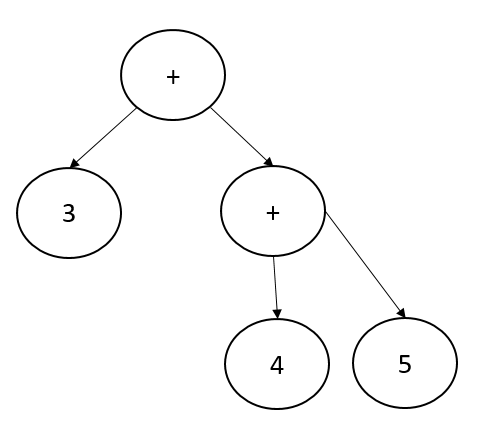
\includegraphics[width=0.4\textwidth]{AST2.png}
	\caption{AST correspondiente a la expresión: \texttt{(+ 3 (+ 4 5))}}
	\label{AS2}
\end{figure}

Una clase en Lisp puede heredar de varias clases \cite{sonya}. Esta característica resulta muy conveniente en el diseño de las jerarquías de nodos del AST y de los lenguajes de salida, lo que se puede observar en la sección \ref{sec:Jerarquía de lenguajes}.

El Sistema de Objetos de Common Lisp utiliza funciones genéricas para especificar las operaciones sobre las instancias de una misma clase \cite{practical-common-lisp}. 

\subsubsection{Funciones Genéricas y Métodos}
Una función genérica define solo una interfaz. Su comportamiento depende de la definición de su Lambda List, y su implementación se distribuye entre un conjunto de métodos\cite{cltl2}.
 
La función genérica que se presenta a continuación, se utiliza en ADOL* \cite{Adol*}, LAML \cite{hoyos} y IVNS \cite{cami} en la etapa de generación de código.
\begin{verbatim}
          (defgeneric generate-code node language stream)
\end{verbatim}

Esta función genérica es la clave para generar código hacia varios lenguajes. Recibe tres parámetros: \texttt{node}, \texttt{language} y \texttt{stream}; y sus métodos se especializan en generar el código correspondiente a cada nodo \texttt{node} del AST, en cada uno de los posibles lenguajes de salida, en un flujo de salida \texttt{stream}.

Por ejemplo, si se quiere generar el código del nodo \texttt{sum-node} en el lenguaje C\#, resulta necesario definir un método que implemente la función genérica \texttt{generate-code} y se especialice en el nodo \texttt{sum-node} y en el lenguaje C\#, como se muestra a continuación:
	
\begin{verbatim}
(defmethod generate-code ((node sum-node)(language csharp) stream)
    (format  stream “~a + ~a”
        (generate-code (left-hand node) language nil)
        (generate-code (right-hand node) language nil)))
\end{verbatim}
En CLOS, los métodos pueden ser extendidos por otros métodos llamados auxiliares\cite{let-over-lambda}. Estos se definen insertando una palabra clave \texttt{(:before, :after o :around)} después de su nombre y especificando el Lambda List del método que extienden \cite{sonya}. Dichos métodos, se utilizan para automatizar las características comunes en la sintaxis de los lenguajes de salida, lo que se ejemplificará en la sección \ref{lenguajesygcode}.

A pesar de ser una herramienta extremadamente poderosa \cite{sonya}, CLOS es solo un DSL interno en Common Lisp para el desarrollo orientados a objetos \cite{sonya}. Este sistema de objetos se pudo incluir en todos los dialectos de Lisp gracias a las funcionalidades del Sistema de Macros que se presentan a continuación.
\subsection{Sistema de Macros}
\label{macros}
Los macros en Lisp son estructuras sintácticas que permiten transformar fragmentos de código Lisp en otros fragmentos de código \cite{Land-of-Lisp}. Aunque los macros están presentes en varios lenguajes de programación como C++ y BASIC, los macros de Lisp trabajan de forma completamente diferente y a un nivel más sofisticado \cite{Land-of-Lisp}.

El Sistema de Macros de Common Lisp constituye una forma de extender la sintaxis del lenguaje \cite{onlisp}. Por ejemplo, en Common Lisp no está definida la sentencia \texttt{while} que posee el lenguaje de programación C\#. Sin embargo, en Common Lisp se puede definir un macro que implemente esta funcionalidad y permita escribir código como:
\begin{verbatim}
                    (while (< x 10)                                  
                       (setf x (+ x 1)))
\end{verbatim}

La instrucción \texttt{while} representa solo una básica sustitución de código, pero con esta idea se pueden crear DSLs para definir iteraciones complejas como el \texttt{Loop} de Common Lisp  \cite{onlisp}, un generador de HTML \cite{ansi-common-lisp} o un intérprete de PROLOG, este último en solo 145 líneas de código \cite{onlisp}.

Los macros se procesan en un tiempo diferente al que se evalúan las funciones o demás operaciones de un programa. Una función en Common Lisp se evalúa cuando se ejecuta un programa que la contenga (\textit{runtime}). Por otro lado, los macros se ejecutan cuando se lee y se compila el programa. Dicho momento se conoce como tiempo de expansión de macros (\textit{macro expansion time}, en inglés). Los parámetros de un macro no se evalúan en el momento en que estos son llamados, sino después de haber compilado el fragmento de código expandido por el macro \cite{onlisp}. La expansión de la llamada anterior al macro \texttt{while} sería:

\begin{verbatim}
                    (loop while (< x 10)
                        doing (setf x (+ x 1)))
\end{verbatim}

En este proyecto, los macros se utilizan para crear funcionalidades que permiten simplificar la creación de nodos del AST, definir automáticamente las funciones constructoras y encapsular fragmentos que se repiten en la generación de código. 

Con los elementos presentados en este capítulo es posible automatizar la creación de Generadores Multilenguajes en Common Lisp. En el siguiente capítulo se describe en detalle el proceso de creación de un Generador Multilenguaje, para posteriormente presentar cómo se puede automatizar cada uno de sus pasos.

%Hasta el momento, han sido presentados conceptos básicos sobre los Generadores Multilenguajes, DSLs, ASTs, así como las propiedades presentes en el Lenguaje de Common Lisp para diseñarlos e implementarlos.\\ 
%


%%% Local Variables:
%%% mode: latex
%%% TeX-master: "../Thesis"
%%% End:

 \chapter{Implementación de un Generador Multilenguaje}
\label{chap:implementacion de un generador }
La implementación de un Generador Multilenguaje se puede dividir en dos etapas fundamentales. Primero, se debe diseñar e implementar el DSL, y luego definir cómo se llevará a cabo la generación de código de cada elemento del dominio en los lenguajes de salida.

A su vez, estas dos etapas se pueden desglosar en un conjunto de pasos lógicos, descritos a continuación:
\begin{enumerate}
	\item Determinar el dominio que se quiere representar en el DSL.
	\item Identificar los elementos que se desean representar en el DSL.
	\item \label{item:diseñar-dsl} Dise\~nar el lenguaje del DSL.
	\item \label{item:jerarquia-de-clases}Implementar una jerarqu\'ia de clases que permita representar cada uno de los elementos del DSL como nodos de un AST.
	\item \label{item:paso-parser-lexer} Construir el analizador lexicogr\'afico y el sint\'actico.
	\item 	\label{item:generacion-de-codigo}Implementar la generaci\'on de c\'odigo de cada uno de los nodos del AST, en cada uno de los lenguajes de salida.
\end{enumerate}

En las siguientes secciones de este capítulo, se ilustran estos pasos a partir de la creación de un Generador Multilenguaje muy simple, cuyo dominio es el trabajo con operaciones aritméticas. A este Generador Multilenguaje se le llamará BASAR (del inglés Basic Arithmetic Operations).

\section{BASAR}

BASAR es un Generador Multilenguaje donde se pueden escribir expresiones aritméticas básicas, que contengan variables y asignaciones a las mismas. Con BASAR se pueden escribir expresiones como:

\begin{verbatim}
                    X = 5 + Y * 2 
\end{verbatim}
Cuando se genere su código a C\#, R, y a Common Lisp se obtendría, respectivamente:
\begin{verbatim}
                    X = 5 + Y * 2;
                    
                    X <- 5 + Y * 2
                    
                    (setf X (+ 5 (* Y 2)))
\end{verbatim}

Una vez que se tiene bien definido el dominio que se quiere representar, el siguiente paso para la construcción de un Generador Multilenguaje es identificar qué elementos del dominio deben ser incluídos.

\section{Dominio}

En el caso de BASAR, los elementos que se desean incluir son: 
\begin{itemize}
\item Suma
\item Multiplicación
\item Asignación a variable
\item Referencia a variable
\item Imprimir
\end{itemize}
Definidos estos elementos, en el siguiente paso se diseña un lenguaje que permita expresar los elementos del dominio.
\section{Lenguaje}
En este paso resulta necesario definir cómo se representa en el DSL cada uno de los elementos del dominio que se quieren incluir. En el caso de BASAR, cada elemento se pudiera representar como se muestra a continuación:
\begin{itemize}
\item   Suma: Será una función \texttt{SUMA} que posee dos parámetros.\\ 
Ejemplo: \texttt{SUMA(A,B)} 
\item   Multiplicación: operador infijo \texttt{*}.\\ Ejemplo: \texttt{A*B}
\item Asignación a variable: operador \texttt{:=}.\\
 Ejemplo: \texttt{A := B}
\item Referencia a variable: nombre de la variable.\\
 Ejemplo: \texttt{A}
\item Imprimir: función Print.\\ 
Ejemplo: \texttt{Print A}
\end{itemize}
Con este diseño del lenguaje, la expresión $X = 5 + Y * 2$ se escribiría: 
\begin{verbatim}
                    X := SUMA(5, Y*2) 
\end{verbatim}
En el caso de \gagm, los DSLs se van a diseñar como lenguajes internos en Common Lisp, por lo que la sintaxis siempre será la misma: todos los elementos se representarían como:

\begin{verbatim}
            (name-funtion arg1, arg2,..., argN).
\end{verbatim}
En este caso solo habría que definir qué nombre tendrá la función que representa a cada uno de los elementos del dominio, de forma que si la asignación se representa por la función \texttt{assign-to}, y la suma y el producto por los operadores \texttt{+}, y \texttt{*}, la expresión $X = 5 + Y * 2$ se representaría como:

\begin{verbatim}
                    (assign-to X (+ 5 (* Y 2))
\end{verbatim}
De esta forma se termina de definir el lenguaje. El siguiente paso es representar cualquier cadena del lenguaje en un AST, lo que se ejemplifica en la próxima sección.

\section{Nodos del Árbol de Sintaxis Abstracta}

Una vez diseñado el lenguaje para un Generador Multilenguaje, se debe crear una jerarquía de clases para los nodos del AST, que dependa de las especificidades del problema. En el caso de BASAR, se define  una clase por cada operación que se desea representar. Además se crea la clase \texttt{binary-operator}, de la que heredan \texttt{sum-node} y \texttt{mult-node}. En la figura \ref{nodos-para-Basar} se muestra la jerarquía de clases para este problema, y en la figura \ref{AST3}, se muestra el AST para el ejemplo de la sección anterior.
\begin{figure}
    \centering
    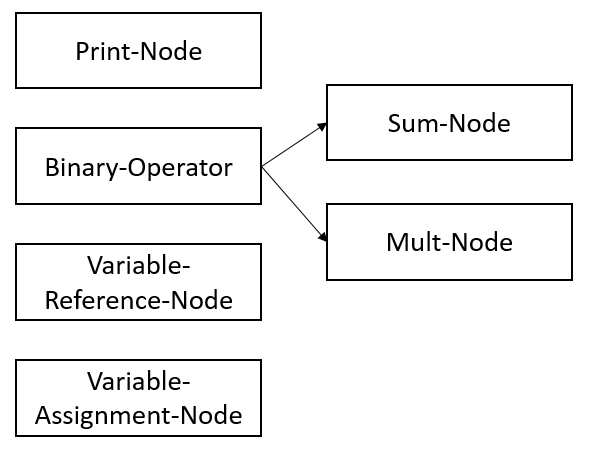
\includegraphics[width=0.5\textwidth]{simple-jerarquia.png}
    \caption{Jeraquía de nodos del AST para BASAR}
    \label{nodos-para-Basar}
\end{figure}
\begin{figure}
    \centering
    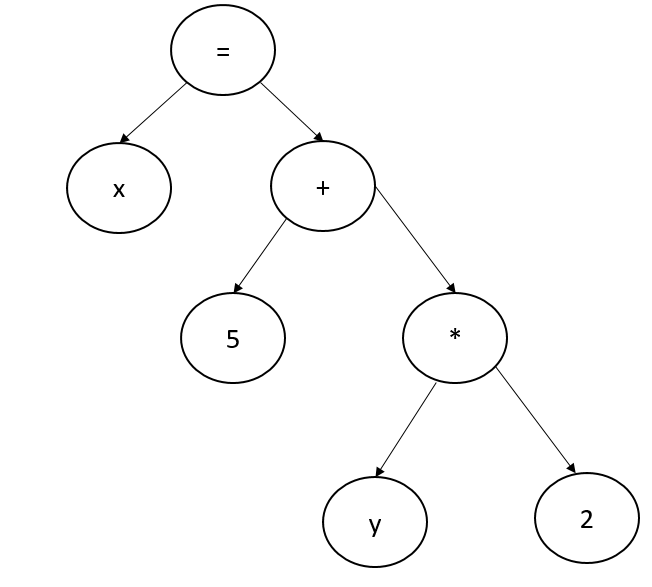
\includegraphics[width=0.5\textwidth]{AST3.png}
    \caption{AST correspondiente a la expresión: (ASSIGN-TO X (+ 5 (* Y 2))}
    \label{AST3}
  \end{figure}

  En dependencia del lenguaje de programación en el que se desee implementar un Generador Multilenguaje, puede ser necesario implementar el analizador lexicográfico y el sintáctico, para construir el AST, a partir de las cadenas del DSL. Como en {\gagm} los lenguajes para los DSLs tendrán la misma sintaxis \texttt{(nombre arg1, arg2, ..., argN)} y los ASTs se pueden obtener mediante funciones constructoras, el intérprete de Common Lisp realizará estos análisis.
  
  Terminada la construcción del AST, se procede a generar el código de sus nodos a los lenguajes de salida.
  
  \section{Generación de código }
  
Para generar el código de programas escritos en BASAR en cualquiera de los lenguajes de salida, basta con especificar cómo se escribe cada nodo del AST en el lenguaje deseado. De esta forma, para escribir el código de un programa completo se recorre el AST que lo representa, generando el código de cada nodo.

Por ejemplo, para escribir en C\# el código correspondiente al AST ilustrado en la figura \ref{AST3}, se necesita especificar cómo generar el código de cada uno de los nodos. Si \texttt{G(X)} representa la generación de código del elemento \texttt{X} se tiene que:

\begin{itemize}
    \item La asignación en C\# es: 
          \begin{verbatim}
             G(parte-izq) = G(parte-der)  
          \end{verbatim}
    \item La suma en C\# es:
     \begin{verbatim}
             G(parte-izq) + G(parte-der)  
     \end{verbatim}
    \item La multiplicación en C\# es:
       \begin{verbatim}
              G(parte-izq) * G(parte-der)  
       \end{verbatim}
    
    \item   La referencia a variable en C\# es:
       \begin{verbatim}
               Nombre-de-la-variable
       \end{verbatim}

    \item Imprimir un elemento en C\#:
     \begin{verbatim}
              Console.WriteLine(G(A))
     \end{verbatim}
    
\end{itemize}  

Una vez definida la generación de código para cada nodo y para cada lenguaje, se puede recorrer el AST generando el código. Los resultados de generar el código del AST ilustrado en \ref{AST3} en C\# y en Common Lisp serían:
\begin{verbatim}
               X = 5 + Y * 2
               
               (setf x (+ 5 (* (Y 2))))
\end{verbatim}

Una de las características principales de un Generador Multilenguaje es que permite definir con facilidad nuevos lenguajes de salida. Por ejemplo, una vez definido el DSL y la generación de código hacia C\#, si se quiere incluir Common Lisp como un lenguaje de salida, solo habría que definir cómo se escribe cada nodo del AST en este nuevo lenguaje.  Si se quisiera hacer la generación de código para otro lenguaje que posea elementos comunes con C\# o Common Lisp, se puede reutilizar la generación de código que ya existe. 

%Common Lisp, puesto que el lenguaje ya está definido. 

Los pasos presentados para desarrollar la implementación de un Generador Multilenguaje serán aplicados en el próximo capítulo, cuando se presente  la herramienta \gagm, que permite agilizar estos pasos.

%Además, dichos pasos también se pueden observar en la implementación de ADOL*.  Independientemente de cual sea su dominio, esta metodología es común para el desarrollo de todos los Generadores Multilenguajes, salvo el caso de identificar los elementos del dominio a representar en su DSL.
 
% En el siguiente capítulo, se aterriza esta metodología para implementar un Generador Multilenguaje en Common Lisp y se identifican fragmentos de código repetidos que serán eliminados utilizando la herramienta propuesta en este trabajo de diploma. Además, se presenta dicha herramienta. 



%%% Local Variables:
%%% mode: latex
%%% TeX-master: "../Thesis"
%%% End:

 \chapter{\gagm}
\label{chap:GAGM}

% \textit{``Mucho de mi trabajo comienza por ser perezoso. No me gusta escribir programas, para que, cuando trabajaba en IBM 701, escribía programas para computar la trayectoria de misiles, yo empecé a trabajar en sistemas de programación que hacían fácil escribir programas''.}


% Cita a John Backus representante del equipo de Desarrollo de IBM que creó Fortran en 1956 

Los Científicos de la Computación estudian para crear programas y algoritmos que minimicen el tiempo de resolución de cualquier problema. Para ello, crean procedimientos y funcionalidades que sean capaces de simplificar procesos mecánicos y repetitivos para el desarrollo de un software. Con esa filosofía, se presenta en este capítulo la herramienta \gagm, para aumentar la eficiencia de los usuarios de Common Lisp en la creación de Generadores Multilenguajes.

En la implementación de un Generador Multilenguaje aparecen fragmentos de código que se repiten con frecuencia, y que pueden ser automatizados utilizando el Sistema de Macros de Lisp y las herramientas que brinda CLOS.  Por ese motivo, en la siguiente sección se presenta una metodología que permite implementar este tipo de programas en Common Lisp. La sección \ref{AST en GAGM} está dedicada a analizar fragmentos de código repetidos durante el diseño de clases y funciones constructoras. Por último, se presenta  la técnica utilizada para generar código hacia distintos lenguajes y patrones que están presentes en su implementación. 

\section{Generación Multilenguaje en \gagm}
\label{chap:Generación Multilenguaje en Gagm}
El desarrollo de Generadores Multilenguajes es el objeto de estudio de este trabajo. En la presente sección se explica cómo puede implementarse este tipo de programa en Common Lisp. 

La metodología presentada a continuación para implementar un Generador Multilenguaje en Common Lisp fue utilizada en la definición de varios programas como: ADOL* \cite{Adol*}, LAML \cite{hoyos} y (IVNS) \cite{cami}. Precisamente, los pasos repetidos en sus implementaciones, son los que se pueden automatizar con la herramienta propuesta en este trabajo.

El grado de dificultad de implementar un programa computacional está condicionado por el lenguaje de programación seleccionado para su desarrollo, ya que cada uno posee características distintas. Independientemente del lenguaje de programación elegido, los pasos a seguir para implementar un Generador Multilenguaje, usualmente son los mismos: 
\begin{enumerate}
	\item Determinar el dominio que se quiere representar en el DSL.
	\item Identificar los elementos que se desean representar en el DSL.
	\item \label{item:diseñar-dsl} Dise\~nar el lenguaje del DSL.
	\item \label{item:jerarquia-de-clases}Implementar una jerarqu\'ia de clases que permita representar cada uno de los elementos del DSL como nodos de un AST.
	\item \label{item:paso-parser-lexer} Construir el analizador lexicogr\'afico y el sint\'actico.
	\item 	\label{item:generacion-de-codigo}Implementar la generaci\'on de c\'odigo de cada uno de los nodos del AST, en cada uno de los lenguajes de salida.
\end{enumerate}

Esta investigación se centra en los pasos 4 y 6, porque los pasos 1 y 2 dependen del dominio específico y se supone que ya han sido realizados. El paso 5 no se tiene en cuenta, debido a que los DSLs serían internos en Common Lisp y sus respectivos lenguajes estarán formados por funciones constructoras, por eso, su mismo intérprete realiza el análisis lexicográfico y el sintáctico. 

En Common Lisp, los elementos identificados en el paso 2 de la lista anterior, se pueden representar con clases, donde los \textit{slots} de cada una son las propiedades de dicho elemento; estas clases representarán los nodos del AST. Los elementos del lenguaje (palabras clave, declaraciones, instrucciones y funciones) pueden ser las funciones constructoras de las clases.  Debido a que estas funciones devuelven instancias de los nodos del AST, y escribir un programa en el DSL consiste en realizar un conjunto de llamados a estas funciones, el resultado de evaluar un segmento de código de ese lenguaje es el AST correspondiente.

Para los usuarios de Common Lisp, implementar un Generador Multilenguaje se traduce en:
\begin{enumerate}
	\item Diseñar una clase para cada elemento del dominio que se quiera representar en el DSL.
	\item Crear una función constructora para cada clase, donde estas funciones constructoras serán los elementos del lenguaje.
	\item Implementar la generación de código de cada uno de los nodos del AST, en cada lenguaje de salida.
\end{enumerate}	

En todos estos pasos aparecen segmentos de código que se repiten. A continuación, se muestran algunos de ellos en la definición de los nodos del AST.

\section{Definición de los nodos del AST}
\label{AST en GAGM}
En la metodología referenciada en la sección \ref{chap:Generación Multilenguaje en Gagm} para implementar Generadores Multilenguajes en Common Lisp, los nodos del AST se obtienen como resultado de evaluar las funciones constructoras de las clases que representan los elementos del DSL. Definir los nodos de un AST en Common Lisp es un proceso mecánico que puede ser automatizado.

Implementar una clase y una función constructora en CLOS se puede ver como dos plantillas  a rellenar. Estas plantillas se rellenan con palabras clave especificadas en Common Lisp e información introducida por el programador para definir una clase o función constructora.  Por ejemplo, la implementación de una clase requiere la palabra clave \texttt{defclass} y la información suministrada por el programador es el nombre de la clase y los \textit{slots} de la misma.

\subsection{Construcción de clases sin \gagm}
\label{patron clases}
Las clases en Common Lisp poseen un patrón común que puede encapsularse utilizando macros. Para ello, se debe identificar la manera en que se escriben sus plantillas. Con el objetivo de mostrar la estructura de dicha plantilla para definir clases, a continuación, se muestra una implementación de las clases \texttt{sum-node}, \texttt{mult-node}, \texttt{variable-assignment-node}, \texttt{variable-reference-node} y \texttt{print-node}; correspondientes a los elementos de BASAR: Suma, Multiplicación, Asignación a Variable, Referencia a variable e Imprimir.


\begin{verbatim}
        (defclass binary-operator ()
               ((left-hand 
                          :accessor left-hand
                          :initarg :left-hand)
                (right-hand 
                          :accessor right-hand 
                          :initarg :right-hand)))
                             
       (defclass sum-node (binary-operator) ())
        
       (defclass mult-node (binary-operator)())    
        
        (defclass variable-assignment-node ()
                  ((variable-name 
                             :accessor variable-name 
                             :initarg :variable-name)
                    (value 
                              :accessor value
                              :initarg :value)))
        
        (defclass variable-reference-node ()
                  ((variable-name 
                              :accessor  variable-name
                              :initarg  :variable-name)))
        
        (defclass print-node ()
             ((value
                          :accessor value
                          :initarg :value)))
\end{verbatim}

Como se puede observar en la implementación anterior, la estructura para rellenar una plantilla de clase en Common Lisp es la siguiente:

Primero, se debe escribir la palabra clave \texttt{defclass}, seguida por el nombre de la clase, una lista con los nombres de sus super clases, y otra con la definición de los \textit{slots}. Cada definición de \textit{slot} posee las palabras clave que identifican las opciones de los \textit{slots} con sus respectivos nombres o valores. Para finalizar, se deben especificar las opciones de las clases, de forma similar a como se realiza con las opciones de los \textit{slots}. 

Usualmente en la definición de los \textit{slots} de las clases, los valores de las opciones de los \textit{slots} \texttt{accessor} y \texttt{initarg}, reciben el mismo nombre que sus correspondientes \textit{slots}. Este patrón se utiliza  en la sección \ref{defnodebasico}. 

Concluida la representación de un elemento del dominio en una clase, se implementa su función constructora. 

\subsection{Funciones constructoras sin \gagm}
\label{sec:patron en funcion}
Para instanciar cualquier tipo de clase, CLOS solo provee la función \texttt{make-instance}. Por este motivo, en el cuerpo de toda función constructora debe existir un llamado a \texttt{make-instance}.

La función \texttt{make-instance} puede ser vista como una plantilla que recibe el nombre de la clase y una lista en la que se asigna a cada \textit{slot} de la clase un valor.   
\begin{verbatim}
              (make-instance 'sum-node 
                         :left-hand  4
                         :right  5))
\end{verbatim}

Conocida la estructura para la función \texttt{make-instance}, se puede crear fácilmente la plantilla de las funciones constructoras. Esta comienza con la palabra clave que identifica el tipo de función constructora (\texttt{defun}) y el nombre elegido para dicha función. Después se especifican sus parámetros en correspondencia con los \textit{slots} de la clase a instanciar. En el resto de la plantilla, el programador debe escribir el cuerpo de la función, que debe incluir un llamado a la función \texttt{make-instance}. A continuación, se implementan las funciones constructoras para las clases \texttt{sum-node}, \texttt{mult-node}, \texttt{variable-assignment-node}, \texttt{variable-reference-node} y \texttt{print-node}.  
\begin{verbatim}
   (defun sum-node (left-hand right-hand)
                 (make-instance 'sum-node 
                       :left-hand left-hand
                       :right-hand right-hand))
          	
   (defun mult-node (left-hand right-hand)
          	    (make-instance 'mult-node 
          	           :left-hand  left-hand
          	           :right-hand  right-hand))	
          
   (defun variable-assignment-node (variable-name value)
          	    (make-instance 'variable-assignment-node
          	           :variable-name variable-name
          	           :value value))
          	                                     
   (defun variable-reference-node	 (variable-name)
          	    (make-instance 'variable-reference-node	
          	           :variable-name variable-name))
          	                                               	                                     
    (defun print-node (value)
          	     (make-instance 'print-node	
          	           :value value))   	                    			        
\end{verbatim}

Nombrando adecuadamente las funciones constructoras y sus parámetros para representar los nodos del AST y combinándolas con las funciones propias de Common Lisp, se pueden crear Generadores Multilenguajes internos con sintaxis y semántica simple. Utilizando estas funciones, desarrollar un Generador Multilenguaje en {\gagm} resultará un proceso sencillo para los usuarios de Common Lisp.

En la sección \ref{patron clases}  se mostró la definición de clases y en la sección \ref{sec:patron en funcion} la definición de funciones constructoras a través de plantillas. Estas plantillas se pueden simplificar si se eliminan las especificaciones de Common Lisp para definir las clases y las funciones. De forma que para diseñar los nodos del AST, solo se escriban los nombres de las clases, los de sus super clases, y los de sus correspondientes \texttt{slots}. Esta idea se utiliza en el macro \texttt{defnode} para automatizar la construcción de clases y funciones constructoras. En la próxima sección se presenta al macro. \texttt{defnode}.   

\subsection{El macro defnode básico}	
\label{defnodebasico}
El tiempo requerido para desarrollar un Generador Multilenguaje aumenta de forma proporcional al número de elementos que se quieran representar en su DSL. 

Como se puede apreciar en las secciones \ref{patron clases} y \ref{sec:patron en funcion}, implementar la clase y la función constructora para cada elemento de un DSL puede requerir muchas líneas de código. Para simplificar este procedimiento se propone utilizar el macro \texttt{defnode} que a partir del nombre de la clase, sus super clases, y sus \textit{slots}, genera automáticamente la definición de la clase y su función constructora. Por ejemplo: 

\begin{verbatim}
(defnode sum-node () (left-hand right-hand))
\end{verbatim}

A partir del código anterior se obtiene:\\ 

\begin{verbatim}
(defclass sum-node ()
             ((left-hand 
                     :accessor left-hand 
                     :initarg :left-hand)
              (right-hand 
                     :accessor right-hand 
                     :initarg :right-hand)))
					 
(defun sum-node (left-hand right-hand)
                (make-instance 'sum-node 
                     :left-hand  left-hand
                     :right-hand right-hand))								 
\end{verbatim}

En la función constructora de \texttt{sum-node}, su nombre y sus parámetros fueron generados en correspondencia con el nombre de la clase y el de sus \textit{slots}. Esto también ocurre cuando se genera el código correspondiente a las opciones de los \textit{slots} de una clase. El código generado por \texttt{defnode} es completamente modificable. En la sección \ref{defnodeavanzado} se presentan las opciones que permiten adaptar este código a las necesidades del usuario.

Similarmente, implementar todas las clases de BASAR y sus correspondientes funciones constructoras sería: 

\begin{verbatim}
(defnode mult-node () (left-hand right-hand))

(defnode variable-assignment-node () (variable-name value))

(defnode variable-reference-node () (variable-name))

(defnode print-node () (value))
\end{verbatim}

Como se puede inferir de la anterior implementación  de las clases que identifican el dominio de BASAR, una representación más elegante para dicho dominio sería construir la clase abstracta \texttt{binary-operator} y definirla como super clase de \texttt{sum-node}, \texttt{mult-node} y \texttt{variable-assignment-node}.   

Utilizar el macro \texttt{defabsnode}, define la clase \texttt{binary-operator} como una clase abstracta:

\begin{verbatim}
(defabsnode binary-operator () (left-hand right-hand))
                    
(defnode sum-node () (binary-operator) ())
                    
(defnode mult-node () (binary-operator) ())
                    
(defnode variable-assignment-node (binary-operator) ())
                    
\end{verbatim}

Existen escenarios complejos cuyo dominio está formado por numerosos elementos. Un ejemplo de ello son los Generadores Multilenguajes ORG-Mode, Markdown o ADOL* que en su definición cuenta con varias clases similares a \texttt{class-definition-node}. La clase \texttt{class-definition-node} fue implementada en ADOL* por la siguiente razón:\\
Si se quiere hacer una biblioteca de Diferenciación Automática \cite{Da}, siempre es necesario definir al menos una clase que posea los campos valor y derivada, y sobrecargar todos los operadores aritméticos. Por ese motivo, un DSL para diseñar bibliotecas de Diferenciación Automática tiene que permitir definir clases y para ello, debe existir en el AST un nodo “Definición de Clases”. Una implementación equivalente a la realizada en ADOL* sería: 

\begin{verbatim}
       (defclass class-definition-node ()
             ((class-name 
                    :accessor class-name 
                    :initarg :class-name)
              (class-parent 
                    :accessor class-parent
                    :initarg :class-parent
                    :initform nil)
              (slots-definition 
                    :accessor slots-definitions 
                    :initarg :slots-definitions
                    :initform '())
             (constructor 
                    :accessor constructor 
                    :initarg :constructor
                    :initform '())
             (operator-overloads 
                    :accessor operator-overloads 
                    :initarg :operator-overloads
                    :initform '())
             (functions-definition 
                    :accessor functions-definitions 
                    :initarg :functions-definitions
                    :initform '())
             (methods-definition 
                   :accessor methods-definitions
                   :initarg :methods-definitions
                   :initform '())))
\end{verbatim}

Igualmente, definir la clase \texttt{class-definition}, y su función constructora sería:
\begin{verbatim}
   (defnode class-definition (instruction-container) 
         (class-name 
          class-parent 
          slots-definitions 
          constructor 
          operator-overloads 
          functions-definitions 
          methods-definitions))
\end{verbatim}

Una vez construido el AST para representar segmentos de código escritos en un DSL, se debe especificar cómo se escribe cada uno de sus nodos en los distintos lenguajes de salida. Esto se realiza en \gagm, utilizando la función genérica que se presenta en la siguiente sección.

\section{Generación de código en \gagm}

La generación de código en {\gagm} está basada en la función genérica \texttt{generate-code}: 
\begin{verbatim}
      (defgeneric generate-code node language stream)
\end{verbatim}
Los métodos que implementan esta función genérica se especializan en generar el código del nodo \texttt{node}, en el lenguaje de salida \texttt{language}, en el flujo de salida \texttt{stream}. Definir cómo se escriben los programas representados en un AST, en un lenguaje de salida dado, requiere agregar un nuevo método a la función genérica \texttt{generate-code} por cada nodo del AST. Por ejemplo, a continuación se muestra cómo se puede implementar la generación de código del nodo \texttt{sum-node} en el lenguaje C\#:

\begin{verbatim}
(defmethod generate-code ((node sum-node) (language csharp)
                                                    stream)
  (format stream “~a + ~a” 
            (generate-code (left-hand node) language nil)
            (generate-code (right-hand node) language nil)))
\end{verbatim}

Un llamado al método \texttt{sum-node} sería: 
\begin{verbatim}
           (generate-code (sum-node 5 3) csharp T) 
\end{verbatim}

En la construcción de estos métodos existe un conjunto de nodos del AST, cuya implementación es un patrón mecánico que puede ser automatizado. La generación de código de un nodo de este conjunto puede verse como una cadena de texto con variables, donde las variables son sustituidas por los resultados de la generación de código de cada uno de sus descendientes en una instancia del AST. En la implementación anterior de la función genérica \texttt{generate-code} para el nodo \texttt{sum-node} se puede observar este patrón, que fue encapsulado por ADOL* en el macro de nombre \texttt{gcode}. Con \texttt{gcode}, el código anterior sería:

\begin{verbatim}
        (gcode sum-node csharp "~a+~a" left-hand right-hand)
\end{verbatim}

Este macro \texttt{gcode} recibe como primer argumento el nodo cuyo código se desea generar (en este caso \texttt{sum-node}), como segundo, el lenguaje de salida (en este caso \texttt{csharp}), como tercero, una cadena válida para la función \texttt{format} \cite{practical-common-lisp} (en este caso \verb "~a+~a" ), y luego un número arbitrario de parámetros que representan los \texttt{slots} que deben ser incluidos en la generación de código (en este caso, \texttt{left-hand} y \texttt{right-hand}).

El uso de \texttt{gcode} deja de ser factible cuando la generación del código de un nodo no cumple exactamente el patrón anterior.

Un ejemplo puede verse en Python, donde la indentación es obligatoria para el correcto funcionamiento de los programas. Por ejemplo, el ciclo \texttt{while} crea un nuevo contexto y las operaciones de su cuerpo requieren cierta indentación.

Si se desea generar el código del nodo \texttt{while} en Python se debe aumentar la indentación de todas las instrucciones que pertenezcan a su cuerpo. Esta situación no es posible expresarla usando el macro \texttt{gcode} definido en ADOL*, y por tanto la única solución es definir explícitamente el método \texttt{generate-code} para este nodo y en el cuerpo del mismo, aumentar la indentación.

Para ampliar la funcionalidad de \texttt{gcode}, en la siguiente sección se presenta otro enfoque que permite utilizarlo en diversos escenarios.

\subsection{El macro gcode de \gagm}
La nueva estructura para el macro \texttt{gcode} permite modificar cualquier parte en la definición del mismo, de forma que sea posible describir la generación de código de cualquier nodo del AST. Por ejemplo, una implementación para escribir el código del nodo \texttt{while} en Python sería: 
\begin{verbatim}
(gcode while python
       ("while (~a):~%" indent "~a~%" deindent) 
       ((condition) (body))) 
\end{verbatim}

Para generar el código del nodo \texttt{while} en Python se utilizan dos listas. La primera, contiene cadenas de texto o código Lisp; y la segunda, listas de \textit{slots}. Por cada cadena de la primera lista se crea una instrucción \texttt{format} con el \texttt{generate-code} de los \textit{slots} en la lista correspondiente, y si no es una cadena, se considera código Lisp y se inserta en la macro expansión del \texttt{gcode}. En el caso del ejemplo anterior, la macro expansión sería:

\begin{verbatim}
(defmethod generate-code ((node while) (lang python) stream)
   (format stream "while (~a):~%"
       (generate-code (condition node) python nil))
   indent
   (format stream "~a"
       (generate-code (body node) python nil))
   deindent
   (format stream "~%" nil))
\end{verbatim}

En este caso, los símbolos \texttt{indent} y \texttt{deindent}, aumentan o disminuyen la indentación de la generación de código escrita en el flujo \texttt{stream}. 

Utilizar el macro \texttt{gcode} y encontrar características sintácticas similares en los lenguajes de programación, hace que extender cualquier Generador Multilenguaje sea un trabajo más sencillo.  

\subsection{Jerarquía de lenguajes}
\label{sec:Jerarquía de lenguajes}
Generar el código de un programa hacia varios lenguajes requiere definir por cada nodo del AST su correspondiente implementación en todos ellos. Representar las propiedades comunes de la sintaxis de los lenguajes de salida y de los nodos de AST en jerarquías de clase puede simplificar este trabajo.

ADOL* y GEMURAL\cite{gemural} implementan distintas jerarquías de clases para la sintaxis de los lenguajes y otra específicamente propia a sus respectivos DSLs. Un subconjunto de las propiedades sintácticas de los lenguajes se representa en ADOL* con las siguientes clases: la clase \texttt{Infix-Languaje}, que describe lenguajes que usan la notación infija para las expresiones aritméticas; la clase \texttt{Camel-Case-Language}, donde las variables y funciones se escriben en formato Camel-Case; \texttt{Indent-Languaje} y \texttt{Symbol-Separated-Language} representan los lenguajes con indentación (espacios en Python y C\#) y separación de instrucciones \texttt{(';' en C\#)}, respectivamente. 

Los lenguajes de programación de propósito general y DSLs para el trabajo matemático, como Matlab, poseen propiedades sintácticas similares para identificar los operadores aritméticos. Por ejemplo, las operaciones suma, multiplicación, división y comparación se representan con los símbolos \texttt{+, *, /, <, > ,} . Estos operadores se pueden agrupar en una clase llamada \texttt{Basic-Operation-Language}.

La herencia múltiple presente en Common Lisp y las jerarquías para representar lenguajes similares, facilitan la generación de código fuente de bibliotecas implementadas en un DSL hacia nuevos lenguajes. Por ejemplo, si se define el lenguaje \texttt{C-like} y se hace heredar de las clases \texttt{Infix-Language}, \texttt{Indent-Language}, \texttt{Symbol-Separated-Languaje} y \texttt{Basic-Operation-Language}, significa que los lenguajes \texttt{C-like} son lenguajes con instrucciones en notación infija, separadas por algún símbolo y que contienen un conjunto de símbolos para representar operaciones aritméticas. Agregar los lenguajes \texttt{C\#} y \texttt{Java} consistiría en definir la clase \texttt{C-like} como super clase de las clases que representan a estos lenguajes, puesto que \texttt{C\#} y Java poseen características comunes a \texttt{C-like}. Luego, solo restaría definir los nuevos elementos que estos lenguajes incorporan y realizarles la correspondiente generación de código hacia \texttt{C\#} o \texttt{Java}.

La organización jerárquica de clases permite reutilizar código de los lenguajes y de nodos del AST definidos. El uso combinado de estructuras jerárquicas y el macro \texttt{gcode} constituyen las principales herramientas para realizar la generación de código a varios lenguajes. En la sección \ref{lenguajesygcode} se enuncian algunas ideas que permiten automatizar las características sintácticas de los lenguajes.

\begin{figure}
	\centering
	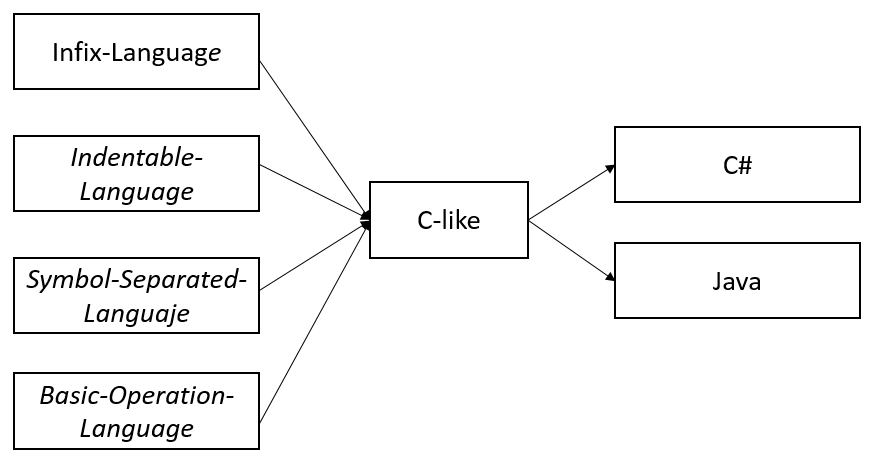
\includegraphics[width=0.6\textwidth]{Adol-jerarquia.png}
	\caption{Jerarquía de lenguajes.}
	\label{Adol8}
\end{figure}

En este capítulo se presentaron las ideas fundamentales para implementar un Generador Multilenguaje en Common Lisp utilizando los macros \texttt{defnode} y \texttt{gcode}. En el próximo capítulo se presentan los principales recursos que permiten cambiar la estructura del código generado por dichos macros. Además se presentan las ideas que permiten automatizar características sintácticas  de los lenguajes de salida.
  


 \chapter{GAGM Avanzada}
\label{chap:GAGMA}

\agregaesto{PON ESTO EN OTRO FICHERO}

Los macros \texttt{defnode} y \texttt{gcode} utilizan la información almacenada en los parámetros de los llamados a dichos macros, para definir las clases, funciones constructoras o realizar la generación de código. Por defecto, si no se especifican las opciones de los slots, las palabras claves, el Lambda List y el cuerpo de las funciones constructoras y de los métodos; esta información será rellenada automáticamente. Debido a que los usuarios pueden necesitar distintas funcionalidades en su dominio, en la próxima sección se presentan otras funcionalidades del macro \texttt{defnode} que permiten modificar el código generado por él. \agregaesto{SI TAMBIÉN VAS A HABLAR DE GCODE, DILO AQUÍ.}

\section{Opciones de DefNode}
\label{defnodeavanzado}
En la definición de las clases y funciones constructoras existen un conjunto de propiedades que Defnode completa con valores prefijados. A continuación, se presentará una opción para definir los slots de las clases y posteriormente las opciones que permiten modificar el código generado por DefNode. 


\agregaesto{NO EMPIECES CON EL LAMBDA LIST DEL DEFNODE NI DE NADA. EXPLICA CON PALABRAS LO QUE QUIERES HACER.}. Lambda List del Defnode:  
\begin{verbatim}
   (Nombre-de-la-clase (lista-de-herencia) (definición-de-slots) 
                       (parámetros-opcionales))
\end{verbatim}

\agregaesto{EL NOMBRE DE LA CLASE Y LA LISTA DE HERENCIA SON IGUALES A LO QUE SE HACE CON EL DEFCLASS, pero en la definición de slots y parámetros opcionales hay cambios. en las siguientes secciones se muestran estos cambios.}

\agregaesto{Vaselina a lo que sigue.}

\subsection{Slots}
Cada elemento de la lista definición-de-slots hace referencia a la declaración de un slot en la definición de la clase Nombre-de-la-clase, y puede ser un símbolo o una lista. Si dicho elemento es un símbolo, la macro expansión de DefNode rellena las opciones ACCESSOR e INITARG con el mismo nombre del slot; si es una lista, se deben definir las opciones de slots que se deseen y sus respectivos valores.  

En el siguiente ejemplo se muestra la definición de una clase con tres slots. 
\begin{verbatim}
        (DefNode collection-definition-node () 
	  	      (collection-name
               collection-type 
	  	       (collection-capacity 
	  	                          :initarg :capacity 
	  	                          :initform 100))
              ())
\end{verbatim}

Los dos primeros serán rellenados con los valores por defecto, pero en el caso del tercero, como se definen dos propiedades el initarg y el initform, esas se agregan a su definición, como se puede apreciar en la macroexpansión del código anterior:

Donde un fragmento de su macro expansión es:
\begin{verbatim}
	     (defclass collection-definition-node () 
	          ((collection-name 
	                 :accessor  collection-name
	                 :initarg  :collection-name 
	                 :allocation instance 
	                 :initform nil 
	                 :documentation “emtpy”)
	           (collection-type 
	                 :accessor  collection-type
	                 :initarg  :collection-type 
	                 :allocation instance 
	                 :initform nil 
	                 :documentation “emtpy”)
	            (collection-capacity 
	                 :accessor collection-capacity
	                 :initarg: capacity
                     :allocation instance
	                 :initform 100
	                 :documentation “empty”))
\end{verbatim}

DefNode emplea un conjunto de palabras claves para agregar o modificar el código que genera su expansión. Ellas son especificadas en el último argumento del Lambda List de dicho macro a través de parámetros nombrados, los cuales se presentan a continuación.

\subsection{Nombre y Tipo de función constructora}
El nombre para la función constructora de una clase se especifica mediante la palabra clave func-name. Las funciones constructoras pueden ser macros, funciones o métodos. A través de la palabra clave ctr-type se especifica el tipo de constructor (defmacro, defun, defmethod).
Ejemplo:
\begin{verbatim}
	(DefNode collection-insert-node () (name value) 
	(:ctr-type funtion :func-name collection-insert))
\end{verbatim}

\subsection{Lambda List de la función constructora}
Por defecto, el Lambda List de las funciones constructoras está formado por los nombres de las opciones Initarg de los slots de la clase a instanciar. Ellos se encuentran ordenados como fueron declarados en su definición.\\ 
Ejemplo:
\begin{verbatim}
	(defnode collection-insert-node () 
	  (collection-name collection-name 
	       (element :initarg :element :initform nil))
	  (:func-name collection-insert)))
\end{verbatim}
Un fragmento de su macro expansión es:
\begin{verbatim}
(defun collection-insert (collection-name  element))
\end{verbatim}
La palabra clave lambda-list permite definir el Lambda List de la función constructora. En este caso, el generado por DefNode se sustituye por la nueva especificación de los parámetros.\\ 
Ejemplo:\\
Si se desea que la clase collection-insert-node reciba un número arbitrario de argumentos, se define su Lambda List como se muestra a continuación.
\begin{verbatim}
(defnode collection-insert-node () (reference-collection value) 
                                   (:ctr-type funtion 
                                    :func-name collection-insert-range 
                                    :lambda-list (&rest value)))
\end{verbatim}
Un fragmento de su macro expansión sería:
\begin{verbatim}
(defun collection-insert-range (&rest value))
\end{verbatim}

Y a partir de esta definición se puede llamar como: \agregaesto{PON UN EJEMPLO DE CÓMO SE LLAMARÍA A LA FUNCIÓN. SERÍA BUENO, UN EJEMPLO DE CÓMO SE PUEDE USAR EL CONSTRUCTOR POR DEFECTO, Y LOS CAMBIOS QUE LE PODEMOS HACER NOSOTROS.}

\subsection{Ctr-body}

El cuerpo de la función constructora se puede especificar con la palabra clave ctr-body.
Ejemplo:
\begin{verbatim}
(defnode collection-insert-node ()(reference-collection value)
								(:ctr-body (make-instance 'collection-insert-node
								               :reference-collection reference-collection)
								               :value value))
\end{verbatim}
En este caso, el valor de ctr-body puede ser cualquier fragmento de código Lisp válido.


%\agregaesto{FINAL DE SECCIÓN}

%%% Local Variables:
%%% mode: latex
%%% TeX-master: "../Thesis"
%%% End:

\backmatter
\begin{conclusions}
En este trabajo se identificaron las principales etapas en la construcción de un Generador Multilenguaje, se presentó una metodología para desarrollar estas aplicaciones en el lenguaje de programación Common Lisp, y se automatizó la escritura de código repetido y mecánico.   

Para automatizar la escritura de código se crearon dos macros fundamentales: \texttt{defnode} que permite automatizar la definición de clases y sus funciones constructoras, y \texttt{gcode}, que simplifica la generación de código, y está inspirado en una funcionalidad similar existente en trabajos anteriores.

Utilizar los macros creados en {\gagm} posibilita escribir, en pocas líneas de código, Generadores Multilenguajes que usualmente necesitan en su implementación grandes cantidades de líneas de código. Con la herramienta presentada en este proyecto, definir el DSL de un Generador Multilenguaje es realizar una selección adecuada de los nombres y de los campos para los elemento de su dominio, y su generación de código hacia los distintos lenguajes se convierte en encontrar patrones que se repiten, encapsularlos, y dedicarse solamente, a escribir el código diferente de cada uno de los elementos de su dominio. 
\end{conclusions}

\begin{recomendations}
	A partir de la investigación realizada se recomienda para trabajos futuros:
	
	\begin{itemize}
		\item Automatizar nuevas características comunes en la sintaxis de los lenguajes de programación.
		\item Añadir a los macros como posibles funciones constructoras.
		\item Agregar nuevas funciones o métodos en la macro expansión de \texttt{defnode}.
	\end{itemize}
\end{recomendations}

%%% Local Variables:
%%% mode: latex
%%% TeX-master: "../Thesis"
%%% End:

% This file was created with JabRef 2.7b.
% Encoding: UTF-8
\bibliographystyle{babplain-uh}
\bibliography{Bibliography}

%% This file was created with JabRef 2.7b.
% Encoding: UTF-8
\printnomenclature


\end{document}
